\documentclass[usenames,dvipsnames]{beamer}
\usepackage{../../shared/styles/custom}
\usepackage{../../shared/styles/conventions}

	\title{Conventions, Accuracy Metrics, Classification, Regression}
\date{\today}
\author{Nipun Batra}
\institute{IIT Gandhinagar}
\begin{document}
%% =============================================================================
% ML TEACHING MATHEMATICAL NOTATION CONVENTIONS
% =============================================================================
% Based on standard ML textbooks: Murphy's "Machine Learning: A Probabilistic Perspective",
% Bishop's "Pattern Recognition and Machine Learning", and "Mathematics for Machine Learning"

% =============================================================================
% CORE NOTATION STANDARDS
% =============================================================================

% SCALARS: Regular italics (lowercase for variables, uppercase for constants)
% Examples: x, y, n, d, k, \theta, \alpha, \lambda, \sigma

% VECTORS: Bold lowercase letters
% Examples: \mathbf{x}, \mathbf{w}, \mathbf{\mu}, \mathbf{\theta}

% MATRICES: Bold uppercase letters
% Examples: \mathbf{X}, \mathbf{W}, \mathbf{\Sigma}, \mathbf{\Lambda}

% SETS: Calligraphic uppercase
% Examples: \mathcal{D}, \mathcal{X}, \mathcal{Y}

% SPACES: Blackboard bold
% Examples: \mathbb{R}, \mathbb{Z}, \mathbb{N}

% =============================================================================
% VECTOR NOTATION (bold lowercase)
% =============================================================================

\providecommand{\vx}{\mathbf{x}}        % Input vector
\providecommand{\vy}{\mathbf{y}}        % Output vector
\providecommand{\vw}{\mathbf{w}}        % Weight vector
\providecommand{\vb}{\mathbf{b}}        % Bias vector
\providecommand{\vh}{\mathbf{h}}        % Hidden vector
\providecommand{\vz}{\mathbf{z}}        % Latent vector
\providecommand{\vf}{\mathbf{f}}        % Function vector
\providecommand{\vg}{\mathbf{g}}        % Gradient vector
\providecommand{\vu}{\mathbf{u}}        % Generic vector u
\providecommand{\vv}{\mathbf{v}}        % Generic vector v
\providecommand{\vzero}{\mathbf{0}}     % Zero vector
\providecommand{\vone}{\mathbf{1}}      % Ones vector

% Greek vectors (bold)
\providecommand{\vmu}{\boldsymbol{\mu}}     % Mean vector
\providecommand{\vtheta}{\boldsymbol{\theta}} % Parameter vector
\providecommand{\vlambda}{\boldsymbol{\lambda}} % Lambda vector
\providecommand{\valpha}{\boldsymbol{\alpha}}   % Alpha vector
\providecommand{\vbeta}{\boldsymbol{\beta}}     % Beta vector
\providecommand{\vxi}{\boldsymbol{\xi}}         % Xi vector
\providecommand{\vepsilon}{\boldsymbol{\epsilon}} % Epsilon vector

% =============================================================================
% MATRIX NOTATION (bold uppercase)
% =============================================================================

\providecommand{\mX}{\mathbf{X}}        % Data matrix
\providecommand{\mY}{\mathbf{Y}}        % Target matrix
\providecommand{\mW}{\mathbf{W}}        % Weight matrix
\providecommand{\mA}{\mathbf{A}}        % Generic matrix A
\providecommand{\mB}{\mathbf{B}}        % Generic matrix B
\providecommand{\mC}{\mathbf{C}}        % Generic matrix C
\providecommand{\mH}{\mathbf{H}}        % Hidden layer matrix / Hessian
\providecommand{\mI}{\mathbf{I}}        % Identity matrix
\providecommand{\mJ}{\mathbf{J}}        % Jacobian matrix
\providecommand{\mK}{\mathbf{K}}        % Kernel matrix
\providecommand{\mL}{\mathbf{L}}        % Loss matrix / Cholesky factor
\providecommand{\mP}{\mathbf{P}}        % Projection matrix
\providecommand{\mQ}{\mathbf{Q}}        % Orthogonal matrix
\providecommand{\mR}{\mathbf{R}}        % Rotation matrix
\providecommand{\mS}{\mathbf{S}}        % Scatter matrix
\providecommand{\mU}{\mathbf{U}}        % Left singular vectors
\providecommand{\mV}{\mathbf{V}}        % Right singular vectors

% Greek matrices (bold)
\providecommand{\mSigma}{\boldsymbol{\Sigma}}   % Covariance matrix
\providecommand{\mLambda}{\boldsymbol{\Lambda}} % Diagonal eigenvalue matrix
\providecommand{\mPhi}{\boldsymbol{\Phi}}       % Feature matrix
\providecommand{\mPsi}{\boldsymbol{\Psi}}       % Basis matrix
\providecommand{\mTheta}{\boldsymbol{\Theta}}   % Parameter matrix

% =============================================================================
% SETS AND SPACES (following Bishop/Murphy conventions)
% =============================================================================

\providecommand{\cD}{\mathcal{D}}       % Dataset
\providecommand{\cH}{\mathcal{H}}       % Hypothesis space
\providecommand{\cX}{\mathcal{X}}       % Input space
\providecommand{\cY}{\mathcal{Y}}       % Output space
\providecommand{\cF}{\mathcal{F}}       % Function space
\providecommand{\cG}{\mathcal{G}}       % Gaussian process
\providecommand{\cL}{\mathcal{L}}       % Lagrangian / Loss
\providecommand{\cN}{\mathcal{N}}       % Normal distribution
\providecommand{\cU}{\mathcal{U}}       % Uniform distribution
\providecommand{\cB}{\mathcal{B}}       % Bernoulli distribution
\providecommand{\cP}{\mathcal{P}}       % Probability distribution

% Number systems
\providecommand{\Real}{\mathbb{R}}      % Real numbers
\providecommand{\Nat}{\mathbb{N}}       % Natural numbers
\providecommand{\Int}{\mathbb{Z}}       % Integers
\providecommand{\Complex}{\mathbb{C}}   % Complex numbers

% =============================================================================
% OPERATORS AND FUNCTIONS (following standard conventions)
% =============================================================================

% Prediction notation (commonly used in ML)
\providecommand{\yhat}{\hat{\vy}}        % Predicted output vector (bold)
\providecommand{\yhati}{\hat{y}_i}       % Predicted output for sample i (scalar)

% Common ML functions (with conflict resolution)
\providecommand{\sigmoid}{}
\renewcommand{\sigmoid}{\operatorname{sigmoid}}
\providecommand{\softmax}{}
\renewcommand{\softmax}{\operatorname{softmax}}
\providecommand{\ReLU}{}
\renewcommand{\ReLU}{\operatorname{ReLU}}
\providecommand{\sign}{}
\renewcommand{\sign}{\operatorname{sign}}
\DeclareMathOperator{\Gain}{Gain}    % Information gain
\DeclareMathOperator{\Entropy}{Entropy}
% KL divergence (check for conflicts)
\providecommand{\KL}{}
\renewcommand{\KL}{\operatorname{KL}}
\DeclareMathOperator{\MSE}{MSE}      % Mean squared error
\DeclareMathOperator{\MAE}{MAE}      % Mean absolute error
\DeclareMathOperator{\RMSE}{RMSE}    % Root mean squared error

% Classification metrics (upright text)
\providecommand{\TP}{\text{TP}}          % True positives
\providecommand{\TN}{\text{TN}}          % True negatives  
\providecommand{\FP}{\text{FP}}          % False positives
\providecommand{\FN}{\text{FN}}          % False negatives
\DeclareMathOperator{\Precision}{Precision}
\DeclareMathOperator{\Recall}{Recall}
\DeclareMathOperator{\Accuracy}{Accuracy}

% Transpose and inverse
\providecommand{\tp}{^\top}             % Transpose (Bishop/Murphy style)
\providecommand{\inv}{^{-1}}            % Matrix inverse
\providecommand{\pinv}{^{\dagger}}      % Pseudoinverse

% Norms (consistent with Murphy/Bishop)
\providecommand{\norm}[1]{\|#1\|}       % Generic norm
\providecommand{\normone}[1]{\|#1\|_1}  % L1 norm
\providecommand{\normtwo}[1]{\|#1\|_2}  % L2 norm
\providecommand{\norminf}[1]{\|#1\|_\infty} % L-infinity norm
\providecommand{\normF}[1]{\|#1\|_F}    % Frobenius norm

% Optimization operators (upright as in Murphy)
\providecommand{\argmin}{}
\renewcommand{\argmin}{\operatorname*{arg\,min}}
\providecommand{\argmax}{}
\renewcommand{\argmax}{\operatorname*{arg\,max}}
\DeclareMathOperator{\minimize}{minimize}
\DeclareMathOperator{\maximize}{maximize}
\DeclareMathOperator{\subjectto}{subject\,to}

% Matrix operations (upright) - use conditional definitions
\providecommand{\tr}{}
\renewcommand{\tr}{\operatorname{tr}}       % Trace
\providecommand{\det}{}
\renewcommand{\det}{\operatorname{det}}     % Determinant
\providecommand{\rank}{}
\renewcommand{\rank}{\operatorname{rank}}   % Rank
\providecommand{\span}{}
\renewcommand{\span}{\operatorname{span}}   % Span
\providecommand{\null}{}
\renewcommand{\null}{\operatorname{null}}   % Null space
\DeclareMathOperator{\range}{range} % Range/column space
\providecommand{\diag}{}
\renewcommand{\diag}{\operatorname{diag}}   % Diagonal operator
\providecommand{\vec}{}
\renewcommand{\vec}{\operatorname{vec}}     % Vectorization operator

% Probability and statistics (Murphy/Bishop style)
\providecommand{\Prob}{\mathbb{P}}      % Probability measure
\providecommand{\Exp}{\mathbb{E}}       % Expectation
\DeclareMathOperator{\Var}{Var}     % Variance
\DeclareMathOperator{\Cov}{Cov}     % Covariance
\DeclareMathOperator{\Corr}{Corr}   % Correlation
% KL divergence already defined above
\DeclareMathOperator{\MI}{I}        % Mutual information

% Activation functions (already defined above with conflict resolution)

% =============================================================================
% STANDARD PARAMETER CONVENTIONS (Murphy/Bishop style)
% =============================================================================

% Primary parameters: θ (theta) - following Murphy's convention
% Learning rates: α, η (alpha, eta)
% Regularization: λ (lambda)
% Precision: β (beta) - following Bishop
% Variance: σ² (sigma squared)
% Standard deviation: σ (sigma)
% Mean: μ (mu)

% Common scalars:
% n - number of training examples
% d - dimensionality of input
% k - number of classes/clusters
% m - number of hidden units
% T - number of time steps
% i, j - indices

% =============================================================================
% STANDARD NOTATION EXAMPLES (Murphy/Bishop style)
% =============================================================================

% Linear regression:      y = \vw\tp\vx + b
% Matrix form:            \vy = \mX\vw + b\vone
% Logistic regression:    p(y=1|\vx) = \sigmoid(\vw\tp\vx)
% Gaussian:               \vx \sim \cN(\vmu, \mSigma)
% Parameter update:       \vtheta_{t+1} = \vtheta_t - \alpha \nabla \cL(\vtheta_t)
% Likelihood:             p(\cD|\vtheta) = \prod_{i=1}^n p(y_i|\vx_i, \vtheta)
% Posterior:              p(\vtheta|\cD) \propto p(\cD|\vtheta)p(\vtheta)
% Prediction:             p(y^*|\vx^*, \cD) = \int p(y^*|\vx^*, \vtheta)p(\vtheta|\cD)d\vtheta

% =============================================================================
% COMMON MISTAKES TO AVOID
% =============================================================================

% ❌ WRONG NOTATION          →  ✅ CORRECT NOTATION (Murphy/Bishop style)

% Transpose:
% ❌ x^t, X^t              →  ✅ \vx\tp, \mX\tp
% ❌ x', X'                →  ✅ \vx\tp, \mX\tp

% Vectors vs Matrices vs Scalars:
% ❌ X (for vector)        →  ✅ \vx (bold lowercase)
% ❌ w (for weight vector) →  ✅ \vw (bold lowercase)
% ❌ x (for data matrix)   →  ✅ \mX (bold uppercase)
% ❌ \mathbf{\theta}       →  ✅ \vtheta (Greek vectors are bold)
% ❌ \mathbf{n}            →  ✅ n (scalars are not bold)

% Sets and distributions:
% ❌ R                     →  ✅ \Real (blackboard bold for number systems)
% ❌ \mathcal{R}           →  ✅ \Real (use blackboard for reals)
% ❌ Normal               →  ✅ \cN (calligraphic for distributions)

% Functions and operators:
% ❌ argmax                →  ✅ \argmax (upright operator)
% ❌ E[X]                  →  ✅ \Exp[X] (blackboard E for expectation)
% ❌ trace(A)              →  ✅ \tr(\mA) (upright operator)

% =============================================================================
% ALGORITHM NAME CONVENTIONS
% =============================================================================

% Use standard capitalizations as in textbooks:
% k-NN, SVM, PCA, GMM, EM, MAP, ML, SGD, Adam, RMSprop
% ReLU, tanh, sigmoid, softmax

\endinput

  % Define counter for pop quizzes

  \maketitle
  
  % Table of Contents
  \begin{frame}{Digit Recognition Problem}
  Let us work on the digit recognition problem.

		\begin{figure}[htp]
			\centering
			\begin{notebookbox}{https://nipunbatra.github.io/ml-teaching/notebooks/rule-based-vs-ml.html}
			  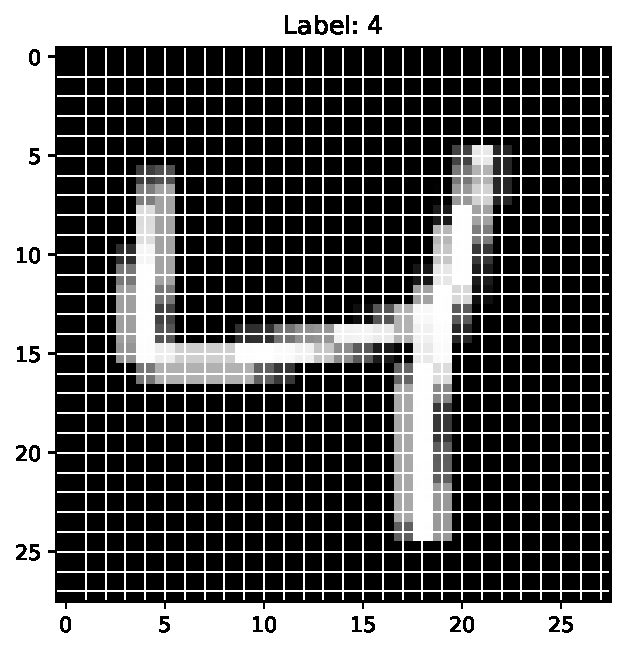
\includegraphics[scale=0.35]{../assets/accuracy-convention/figures/mnist.pdf}
			\end{notebookbox}
		  \end{figure}

	\end{frame}

\begin{frame}{Rule-based Approach for Digit Recognition}
Maybe 4 can be thought of as: $\bm{|}$ + $\bm{\rule[0.5ex]{1em}{.95pt}}$ + $\bm{|}$ + another vertically down $\bm{|}$

\begin{itemize}
	\item \pause The heights of each of the $\bm{|}$ need to be similar within tolerance
	
	\item \pause Each of the $\bm{|}$ can be slightly slanted. Similarly the horizontal line can be slanted.
	\item \pause There can be some cases of 4 where the first $\bm{|}$ is at 45 degrees
	\item \pause There can be some cases of 4 where the width of each stroke is different
	
\end{itemize}

\end{frame}	

\section{Machine Learning Fundamentals}

\begin{frame}{Apple Quality Features}
\begin{itemize}
	\item Size
	\item \pause Colour
	\item \pause Texture
\end{itemize}
\end{frame}
  
\begin{frame}{Should We Include Sample Numbers?}
Answer: Usually no! Sample numbers are typically arbitrary identifiers and not meaningful features. Let us remove it.

\pause Let us modify our data table for now.

\begin{table}[]
	\begin{tabular}{|l|l|l||l|}
		\hline 
		\textbf{Colour} & \textbf{Size} & \textbf{Texture} & \textbf{Condition} \\ \hline 
		Orange & Small & Smooth  & Good      \\
		Red    & Small  & Rough  & Good \\
		Orange & Medium & Smooth & Bad \\
		Yellow & Large  & Smooth & Bad \\ \hline 

	\end{tabular}
\end{table}
\end{frame}

\begin{frame}{Training Set Components}
The training set consists of two parts:
\begin{enumerate}
	\item \pause \color{Lavender}{Features (Input Variables)}
	\item \pause \color{Tan}{Output or Response Variable}
\end{enumerate}
\end{frame}

\begin{frame}{Dataset Notation}
We call this matrix as $\cD$, containing:
\begin{enumerate}
	\item Feature matrix ($\mX \in \Real^{n \times d}$) containing data of $n$ samples each of which is $d$ dimensional.
	\item Output vector ($\vy \in \Real^n$) containing output variable for $n$ samples.
\end{enumerate}

\end{frame}

\begin{frame}{Dataset Example}
Example (after encoding): $\vx_1 = \begin{bmatrix}
	1 \\ 
	0 \\
	1 \\
	\end{bmatrix}$ (Orange=1, Small=0, Smooth=1)

\begin{itemize}
	\item \pause Complete dataset: $\cD = \{(\vx_i\tp, y_i)\}_{i=1}^n$
\end{itemize}

\end{frame}

\begin{frame}{Machine Learning Goal}
Learn $f$: 		$\text{Condition} = f(\text{colour, size, texture})$

\begin{enumerate}
	\item \pause From Training Dataset
	\item \pause To Predict the condition for the Testing set
\end{enumerate}

\begin{table}[]
	\begin{tabular}{|l|l|l||l|}
		\hline 
		
		\textbf{Colour} & \textbf{Size} & \textbf{Texture} & \textbf{Condition} \\ \hline 
		Orange & Small & Smooth  & Good      \\
		Red    & Small  & Rough  & Good \\
		Orange & Medium & Smooth & Bad \\
		Yellow & Large  & Smooth & Bad \\ \hline
		Red    & Large  & Rough  & ? \\
		Orange &  Large & Rough  & ? \\ \hline          
	\end{tabular}
\end{table}
\end{frame}

\begin{frame}{Can We Judge Performance Only on Test Set?}
A: Ideally, no!

\begin{itemize}
	\item \pause Ideally - we want to predict ``well'' on all possible inputs. But, can we test that?
	\item \pause No! Since, the test set is only a sample from all possible inputs.
\end{itemize}

\end{frame}

\begin{frame}{Training vs Test Sets}
Both the training set and the test set are samples drawn from the hidden true distribution (also sometimes called population)

\pause More discussion later once we study bias and variance
\end{frame}

\begin{frame}{Energy Consumption Example}
\begin{itemize}
	\item \# People (More people $\implies$ More Energy)
	\item \pause Temperature (Higher Temp. $\implies$ Higher Energy)
\end{itemize}

\pause \begin{table}[]
	\begin{tabular}{|l|l||l|}
		\hline 
		
		\textbf{\# People} & \textbf{Temp (C)} &  \textbf{Energy (kWh)} \\ \hline 
		
		4000 & 30 & 30 \\
		4200 & 30 & 32 \\
		4200 & 35 & 40 \\ \hline
		3000 & 20& ? \\
		1000 & 45 & ? \\ \hline          
	\end{tabular}
\end{table}
\end{frame}

\section{Classification vs Regression}

\begin{frame}{Classification vs Regression}
\begin{itemize}
	\item Classification
	\begin{itemize}
		\item \pause Output variable is discrete
		\item \pause i.e.  $y_i \in \{1, 2, \ldots, k\}$ where $k$ is number of classes 
		\item \pause Examples - Predicting: 
		\begin{itemize}
			\item \pause Will I get a loan? (Yes, No)
			\item \pause What is the quality of fruit? (Good, Bad)
		\end{itemize}
	\end{itemize}
	\item \pause Regression
	\begin{itemize}
		\item \pause Output variable is continuous
		\item \pause i.e.  $y_i \in \Real$ 
		\item \pause Examples - Predicting: 
		\begin{itemize}
			\item \pause How much energy will campus consume? 
			\item \pause How much rainfall will fall?
		\end{itemize}
	\end{itemize}
\end{itemize}

\end{frame}

%\captionsetup[subtable]{labelformat=empty}
%
\begin{frame}{Accuracy Calculation}
\[
\text{Accuracy} = \frac{|\{i : y_i = \hat{y}_i\}|}{n} = \frac{3}{5} = 0.6
\]
\end{frame}

\begin{frame}{Accuracy Notation}
\begin{itemize}
	\item \textbf{Set cardinality notation:} $|\{i : y_i = \hat{y}_i\}|$ 
	\begin{itemize}
		\item Reads as: ``Number of indices $i$ such that $y_i = \hat{y}_i$''
		\item Counts how many samples satisfy the condition
	\end{itemize}
	
	\item \pause \textbf{Alternative: Indicator function notation}
	\begin{align*}
	\text{Accuracy} &= \frac{\sum_{i=1}^n \mathbf{1}[y_i = \hat{y}_i]}{n}
	\end{align*}
	where $\mathbf{1}[\text{condition}] = \begin{cases} 1 & \text{if condition is true} \\ 0 & \text{if condition is false} \end{cases}$
	
	\item \pause Both notations are mathematically equivalent and commonly used in ML literature
\end{itemize}
\end{frame}

\begin{frame}{When Precision/Recall Matter}
Cases for this:
\begin{itemize}
\item Cancer Screening
\item Planet Detection
\end{itemize}

\end{frame}

\begin{frame}{Precision Metric}
\begin{align*}
\text{Precision} &= \frac{|\{i : y_i = \hat{y}_i = \text{Good}\}|}{|\{i : \hat{y}_i = \text{Good}\}|} = \frac{2}{4} = 0.5
\end{align*}

``the fraction of relevant instances among the retrieved instances'', i.e. ``out of the number of times we predict \text{Good}, how many times is the condition actually \text{Good}''

\end{frame}

\begin{frame}{Accuracy vs Precision/Recall}
\begin{align*}
\text{Accuracy} &= \frac{98}{100} = 0.98 \\
\text{Recall} &= \frac{0}{1} = 0 \\
\text{Precision} &= \frac{0}{1} = 0
\end{align*}

\end{frame}

\begin{frame}{Confusion Matrix}
\vspace{60pt}
\begin{center}
\begin{tabular}{@{}cc cc@{}}
	\multicolumn{1}{c}{} &\multicolumn{1}{c}{} &\multicolumn{2}{c}{Ground Truth} \\ 
	\cmidrule(lr){3-4}
	\multicolumn{1}{c}{} & 
	\multicolumn{1}{c}{} & 
	\multicolumn{1}{c}{Yes} & 
	\multicolumn{1}{c}{No} \\ 
	\cline{2-4}
	\multirow[c]{2}{*}{\rotatebox[origin=tr]{90}{Predicted}}
	& Yes  & True Positive & False Positive   \\[1.5ex]
	& No  & False Negative   & True Negative \\ 
	\cline{2-4}
\end{tabular}
\end{center}
\end{frame}

\begin{frame}{Example Metrics}
\[
\bordermatrix{&\text{G.T. Positive}&\text{G.T. Negative}\cr
               \text{Pred Positive}&0&1\cr
               \text{Pred Negative}&1&98}
\]

\pause
\[
\bordermatrix{&\text{G.T. Positive}&\text{G.T. Negative}\cr
               \text{Pred Positive}&\text{True Positive}&\text{False Positive}\cr
               \text{Pred Negative}&\text{True Negative}&\text{False Negative}}
\]

\pause
\begin{align*}
\text{Recall} &= \frac{\text{T.P}}{\text{T.P + F.P}} \\
\text{Precision} &= \frac{\text{T.P}}{\text{T.P + F.N}}
\end{align*}
\end{frame}


\begin{frame}{Mean Error Issues}
Is there any downside with using mean error?
\pause Errors can get cancelled out

\end{frame}

\section{Data Visualization and Baselines}

\begin{frame}{Pop Quiz}
\begin{popquizbox}{1}
Which metrics should you use for imbalanced datasets?
\begin{enumerate}
\item Accuracy only  
\item Mean squared error
\item Precision, recall, and F1-score
\end{enumerate}

\vspace{0.5em}
\textbf{Answer:} c) Precision, recall, and F1-score give a more complete picture!
\end{popquizbox}
\end{frame}

\begin{frame}{Key Takeaways}
\begin{itemize}
\item \textbf{ML vs Traditional Programming:} ML learns rules from data, traditional programming uses predefined rules
	\pause
\item \textbf{Features matter:} Choose meaningful features, avoid arbitrary identifiers
	\pause
\item \textbf{Classification vs Regression:} Discrete outputs vs continuous outputs
	\pause
\item \textbf{Accuracy isn't everything:} For imbalanced data, use precision, recall, F1-score
	\pause
\item \textbf{Visualization is crucial:} Always plot your data (Anscombe's Quartet lesson)
	\pause
\item \textbf{Use baselines:} Simple baseline models help validate your approach
\end{itemize}
\end{frame}

\begin{frame}{Summary: Evaluation Metrics}
\begin{center}
\begin{tabular}{|l|l|l|}
\hline
\textbf{Task} & \textbf{Common Metrics} & \textbf{When to Use} \\
\hline
\textbf{Classification} & Accuracy, Precision, Recall, F1 & Balanced/Imbalanced data \\
 & Confusion Matrix & Multi-class problems \\
\hline
\textbf{Regression} & MSE, RMSE, MAE & Continuous predictions \\
 & Mean Error & Check for bias \\
\hline
\end{tabular}
\end{center}

\vspace{1cm}
\textbf{Remember:} Choose metrics based on your problem's characteristics and business requirements!
\end{frame}

\end{document}
